% !TEX root = ../../semexp-thesis.tex

\section{Semantic Suggestions}
\label{sec:implementation/suggestions}

We implement semantic suggestions through a \emph{suggestion space} window that is placed as a vertical docking bar at the edge of the screen~(\cref{fig:implementation/suggestions/space}).
To track the experiments of programmers, we observe their mouse and keyboard focus by using Morphic's event filter mechanism.
From the focused windows, we extract the currently browsed classes and methods or drafted scripts and notes as input artifacts for the suggestion engine.

\begin{figure}
	\centering
	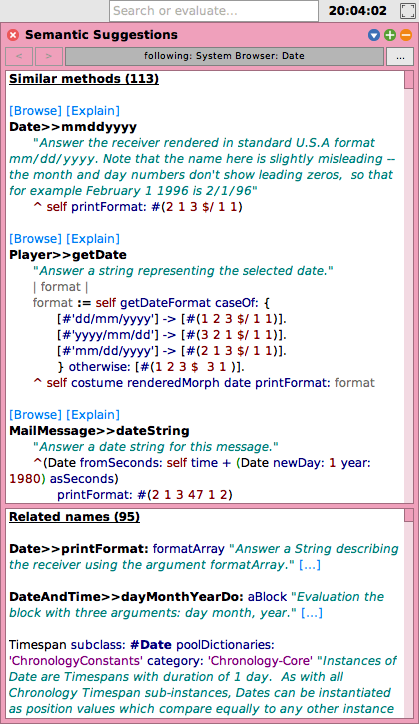
\includegraphics[height=30\baselineskip]{01_suggestions/space.png} % TODO screenshot: [COULD] improve resolution.
	\caption[The user interface of our \emph{suggestion space} for displaying semantic suggestions in Squeak.]{
		The user interface of our \emph{suggestion space} for displaying semantic suggestions in Squeak.
		It is docked to the side of the screen, tracks browsing and editing activities of programmers, and automatically displays suggested artifacts in separate panes.
		Programmers can derive inspiration from suggestions for their own applications or use the ``browse'' buttons to explore individual artifacts.
		Through the ``$\,{\cdots}\,$'' menu, they can customize used strategies and displayed types of artifacts in the suggestion space.
	}
	\label{fig:implementation/suggestions/space}
\end{figure}

In the suggestion space, we display similar code and documentation artifacts, correlated code artifacts, and an optional summary of them.
Suggestions are updated continuously in the background as the programmer conducts experiments by browsing methods or writing code or notes.

To enable semantic retrieval of all classes and methods in the image, we maintain either of them in a semantic corpus~(i.e., a vector store of \semtex).
\footnote{We truncate methods to their first \num{10000} characters to exclude ``data methods'' that define constants such as multimedia data, since they might exceed the context window of the embedding model and rarely contain interesting, human-readable information. While a typical Smalltalk image still contains many shorter data methods, this heuristic already reduced the token consumption of the embedding model by approximated \qty{13}{\percent} in our experiments.}
We subscribe to the \code{SystemChangeNotifier} interface to incorporate updates from the system.
We compute embeddings for new documents asynchronously in the background after the current world cycle has ended (i.e., \code{[aCorpus computeEmbeddings] future forkAt: Processor systemBackgroundPriority}).
This strategy allows for bulk-updating the corpus and avoiding the overhead of multiple requests to the OpenAI API after many code changes have been applied as part of a single operation (such as installing a package).
At the same time, corpus updates are run in the background without noticeable lags.
